\documentclass[border=10pt]{standalone}
\usepackage[svgnames]{xcolor}
\usepackage{amsmath}
\usepackage{pgfplots}
\pgfplotsset{compat=newest}
\usepackage[sfdefault]{FiraSans}
\usepackage{FiraMono}
\renewcommand*\familydefault{\sfdefault}
\begin{document}
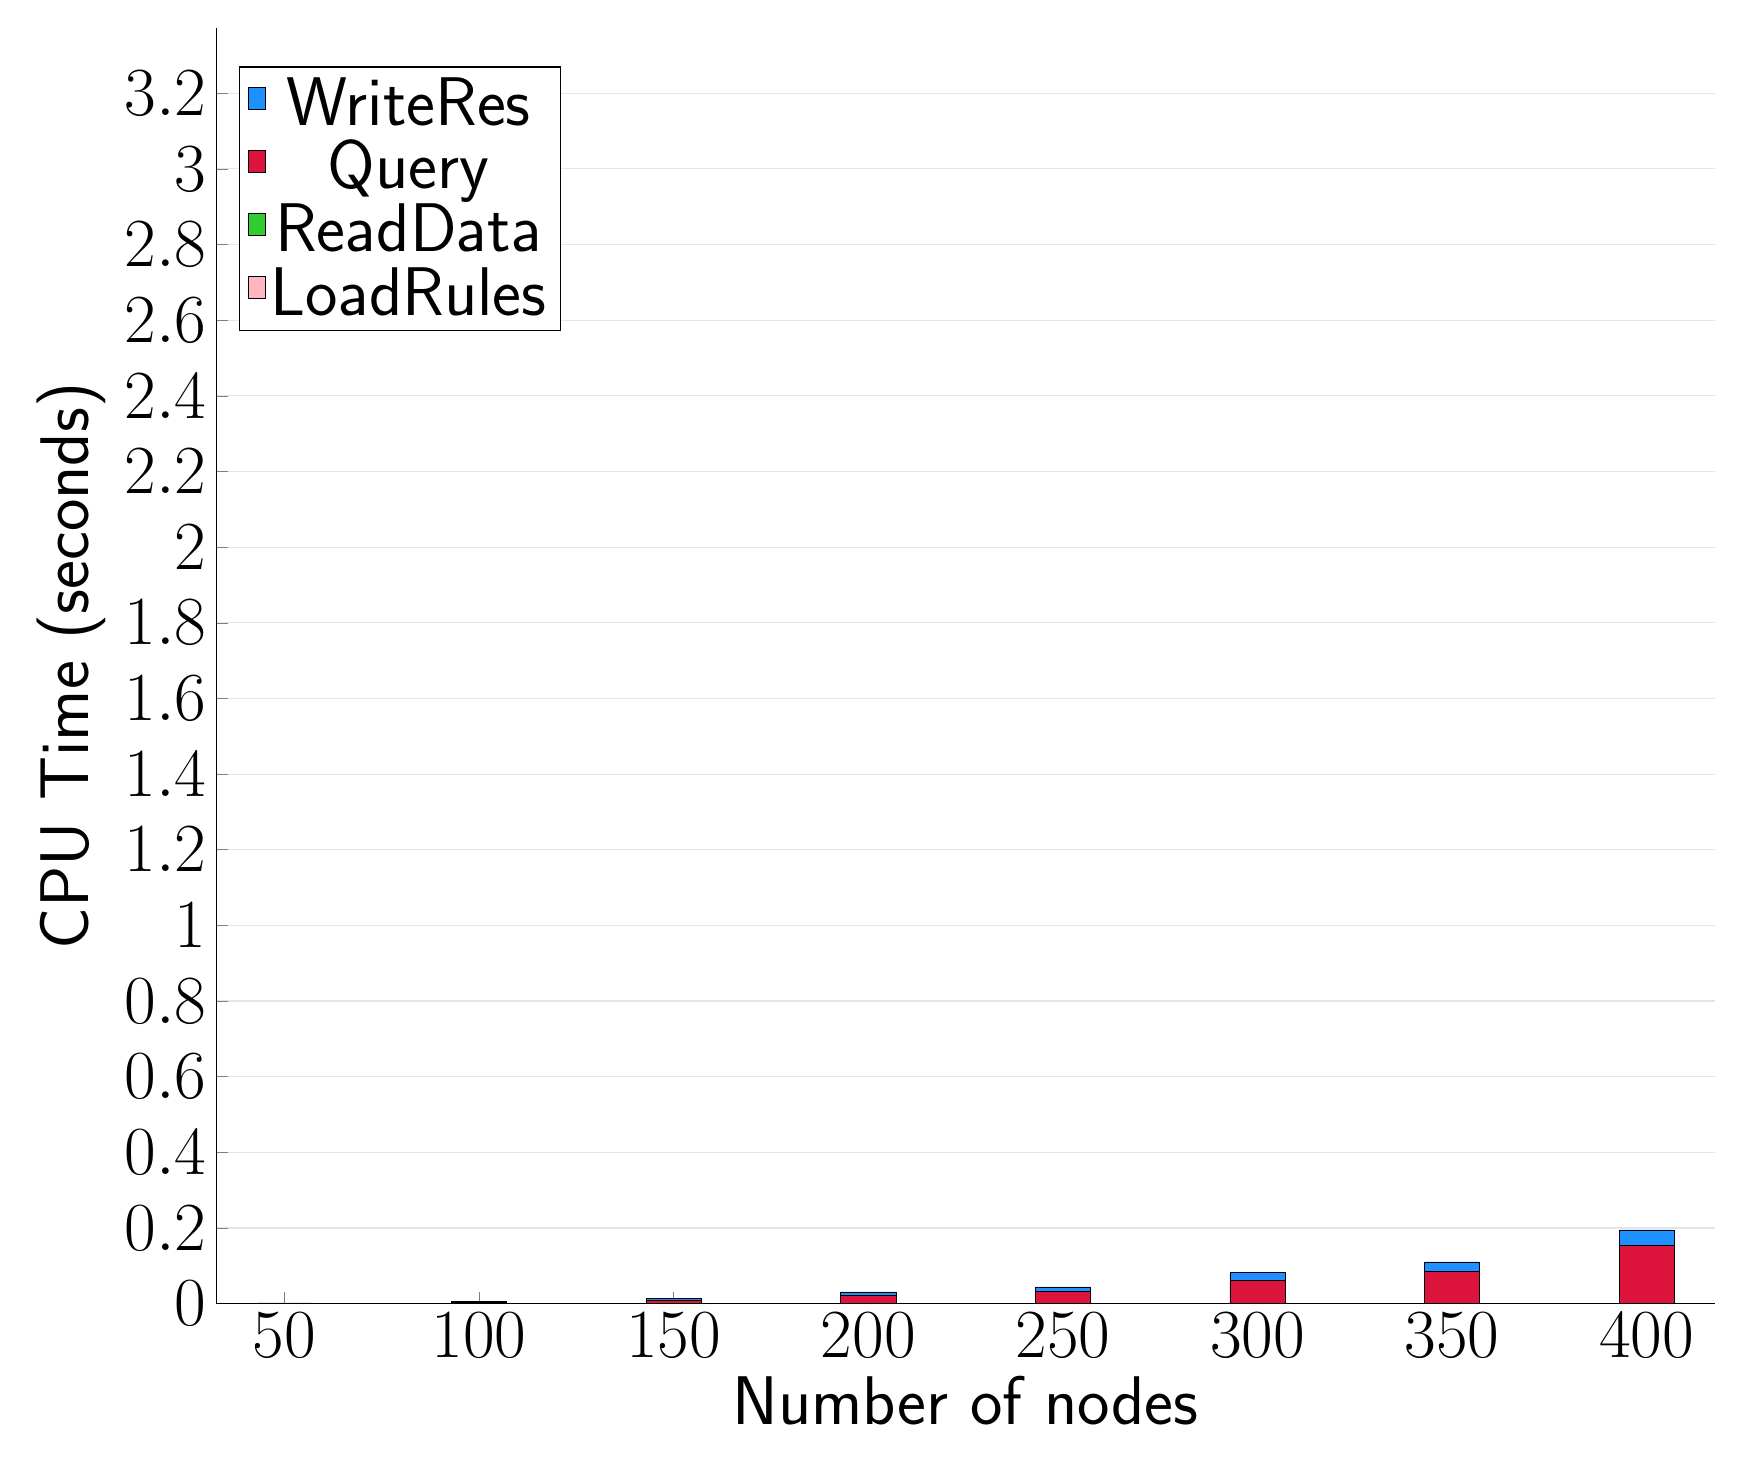
\begin{tikzpicture}
\begin{axis}[
   ybar stacked,
   width=1.7\textwidth,
   bar width=0.7cm,
   ymajorgrids, tick align=inside,
   major grid style={draw=gray!20},
   xtick=data,
   ymin=0, ymax=3.3720000000000003,
   axis x line*=bottom,
   axis y line*=left,
   enlarge x limits=0.05,
   legend style={
       at={(0.23, 0.97)},
       anchor=north east,
       legend columns=1,
       font=\Huge,
   },
   ylabel={CPU Time (seconds)},
   xlabel={Number of nodes},
   label style={font=\Huge},
   tick label style={font=\Huge},
]
\addlegendimage{fill=DodgerBlue, draw=black, line width=0.2pt}
\addlegendentry{WriteRes}
\addlegendimage{fill=Crimson, draw=black, line width=0.2pt}
\addlegendentry{Query}
\addlegendimage{fill=LimeGreen, draw=black, line width=0.2pt}
\addlegendentry{ReadData}
\addlegendimage{fill=LightPink, draw=black, line width=0.2pt}
\addlegendentry{LoadRules}
\addplot +[fill=LightPink, draw=black, line width=0.2pt] coordinates {
(50, 0.0006374999999999995)
(100, 0.0006148000000000002)
(150, 0.0006026000000000001)
(200, 0.0006316000000000006)
(250, 0.0006133000000000004)
(300, 0.0006089000000000007)
(350, 0.0006050000000000002)
(400, 0.0006096999999999995)
};
\addplot +[fill=LimeGreen, draw=black, line width=0.2pt] coordinates {
(50, 0.0002209000000000006)
(100, 0.0002868000000000001)
(150, 0.00035640000000000004)
(200, 0.0004567999999999994)
(250, 0.0004945999999999998)
(300, 0.0006055999999999995)
(350, 0.0006771999999999999)
(400, 0.0007857999999999997)
};
\addplot +[fill=Crimson, draw=black, line width=0.2pt] coordinates {
(50, 0.0004575999999999997)
(100, 0.0030108)
(150, 0.0083033)
(200, 0.0202289)
(250, 0.030231100000000004)
(300, 0.059918799999999994)
(350, 0.08338500000000001)
(400, 0.15335130000000002)
};
\addplot +[fill=DodgerBlue, draw=black, line width=0.2pt] coordinates {
(50, 0.0007342000000000003)
(100, 0.0027848)
(150, 0.0055319)
(200, 0.009837799999999999)
(250, 0.0127906)
(300, 0.0204645)
(350, 0.025584600000000002)
(400, 0.040078499999999996)
};
\end{axis}
\end{tikzpicture}

\end{document}
